\section{Entrer les valeurs restantes/Vue d'ensemble}Ici, vous voyez une vue d'ensemble de tous les postes client \`a cr\'eer. Maintenant, vous pouvez remplir les blancs dans les tables ou les changer et voir si les valeurs correspondent \`a vos id\'ees.\\
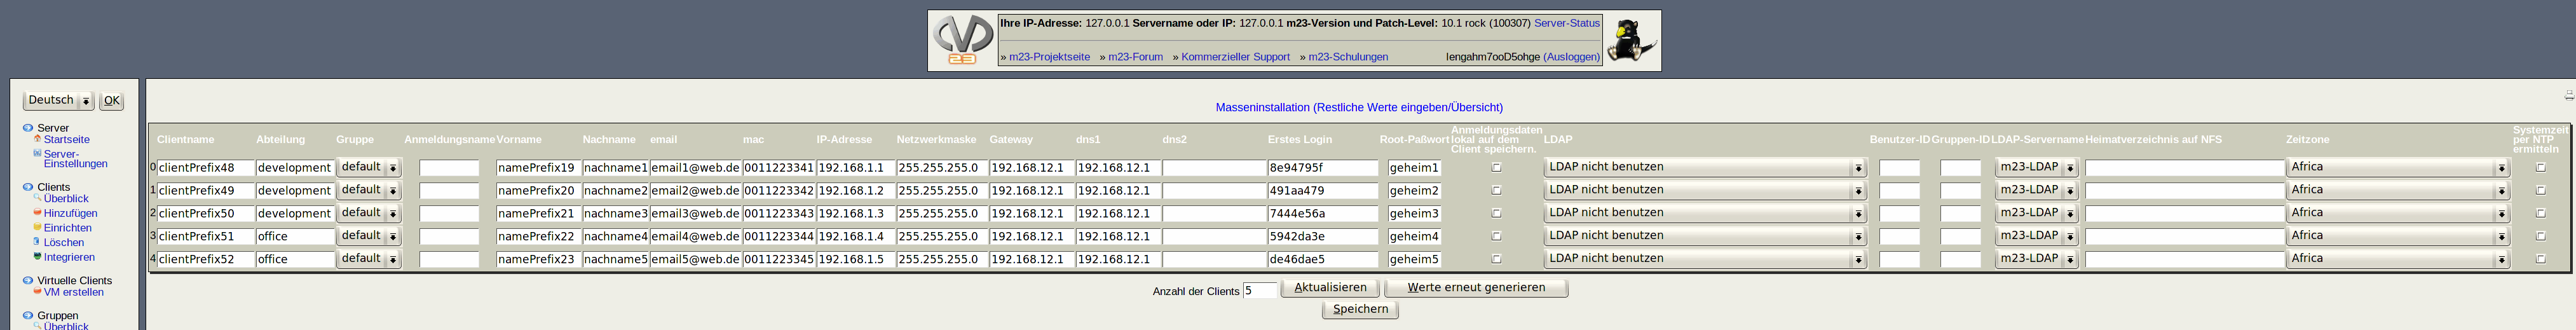
\includegraphics[scale=0.33]{/mdk/doc/manual/screenshots/fr/mi_step4.png} \\
\subsection{Changer le nombre de postes client}
Vous pouvez changer le nombre de postes client en entrant le nouveau nombre chez $\ll$Nombre de postes clients$\gg$ et puis, cliquant sur $\ll$Actualiser$\gg$, si vous d\'esirez avoir moins de postes client ou sur $\ll$G�n�rer les valeurs de nouveau$\gg$, si vous d\'esirez avoir plus de postes client.\\
Si vous d\'esirez un plus grand nombre de postes client qu'auparavant, les g\'en\'erateurs vont g\'en\'erer les valeurs n\'ecessaires apr\`es un clic sur $\ll$G�n�rer les valeurs de nouveau$\gg$ et essayer de lire les autres valeurs du fichier de banque de donn\'ees. Si le fichier de la banque de donn\'ees ne contient pas assez de valeurs, vous devez les entrer manuellement dans la table. La g\'en\'eration d'un grand nombre de valeurs peut peut-\^etre durer un long temps, par exemple si les adresses IP sont en train d'\^etre g\'en\'er\'ees et vous avez choisi que les adresses IP doivent \^etre contact\'ees avant l'usage.\\
Enfin, cliquez sur $\ll$Enregistrer$\gg$ pour commencer avec l'installation sur les postes client.\\
